%@AUTHOR: Cardel
%Configuracion del documento

\documentclass{beamer}
\usetheme{Berkeley}
\setbeamertemplate{caption}[numbered]
\usepackage{graphicx}
\usepackage[utf8]{inputenc}
\usepackage[spanish]{babel}
\usepackage{ragged2e}
\usepackage{colortbl}
\usepackage{color}
\definecolor{naranja}{rgb}{1,0.5,0} % valores de las componentes roja, verde y azul (RGB)
\definecolor{rojo}{rgb}{1,0,0}
\definecolor{SteelBlue}{rgb}{0.3,0.5,0.7}
\usepackage{float}

\author{Carlos Andr\'es Delgado S.} 
\title{710193M Arquitectura de computadores II}
\subtitle{Control microprogramado \\ carlos.andres.delgado@correounivalle.edu.co}
\institute{Facultad de Ingeniería. Universidad del Valle}
%Transparencia
\setbeamercovered{transparent}

%LOGO Univalle
\pgfdeclareimage[height=1.4cm]{logo}{imagenes/univalle}
\logo{\pgfuseimage{logo}}

\usepackage{listings}% http://ctan.org/pkg/listings
\usepackage{listingsutf8}

\lstset{ %
  basicstyle=\footnotesize,           % the size of the fonts that are used for the code
  numbers=none,
  numberstyle=\footnotesize,          % the size of the fonts that are used for the line-numbers
  numbersep=4pt,                  % how far the line-numbers are from the code
  backgroundcolor=\color{white},      % choose the background color. You must add \usepackage{color}
  breaklines=true,                % sets automatic line breaking
  breakatwhitespace=true,        % sets if automatic breaks should only happen at whitespace
  title=\lstname,                   % show the filename of files included with \lstinputlisting;{}
  extendedchars=false,
  inputencoding=utf8, 
  tabsize=2,
   mathescape=true,
  literate={\ \ }{{\ }}1
}
\newsavebox{\myLst}
\newsavebox{\myLstb}
\newsavebox{\myLstc}
\newsavebox{\myLstd}

\usepackage{enumitem} % enumerados

%Para que en cada seccion aparezca la tabla de contenido
\AtBeginSection[]{
	\begin{frame}
	\frametitle{Contenido}
	\tableofcontents[currentsection]
\end{frame}
}




\date{Mayo de 2016}
\newcommand{\grad}{\hspace{-2mm}$\phantom{a}^{\circ}$}
\begin{document}

\begin{frame}
	\titlepage	 		
\end{frame}

\begin{frame}
	\tableofcontents	 		
\end{frame}


\section{Conceptos básicos}

\begin{frame}
	\frametitle{Conceptos básicos}
	\begin{block}{Conceptos}
	\begin{enumerate}
		\item Alternativa a la implementación cableada
		\item Secuencia de instrucciones en un lenguaje de microprogramación
		\item Conexiones sencillas para el secuenciamiento de instrucciones en la CPU
		\item Las microinstrucciones generan las señales de control para las operaciones de la ALU y de transferencias en los registros
	\end{enumerate}
	\end{block}	
\end{frame}


\begin{frame}
	\frametitle{Conceptos básicos}
	\begin{block}{Microinstrucciones}
	\begin{enumerate}
		\item Cada microoperación es descrita en notación simbólica
		\item El conjunto de microoperaciones es denominado como \textbf{lenguaje de microprogramación}
		\item Una secuencia de instrucciones es conocido como microprograma o \textit{firmware}
		\item En la unidad de control, se construye una \textbf{palabra de control}, donde cada bit representa una línea de control y una instrucción es una secuencia de palabras de control
	\end{enumerate}
	\end{block}	
\end{frame}

\begin{frame}
	\frametitle{Conceptos básicos}
	\begin{block}{Tipos de microinstrucciones}
	\begin{enumerate}
		\item \textbf{Microinstrucciones horizontales:} Son microinstrucciones donde cada palabra de control tiene dirección única en memoria, indicando la dirección de la siguiente palabra de control a ejecutar si determinada condición es cierta.
		\item \textbf{Microinstrucciones verticales:} Son microinstrucciones donde cada palabra de control tiene los códigos de función (lo que debe hacer) y la dirección de la siguiente palabra de control a ejecutar si determinada condición es cierta.		
	\end{enumerate}
	\end{block}	
\end{frame}

\begin{frame}
	\frametitle{Conceptos básicos}
	\begin{block}{Tipos de microinstrucciones}
	En la siguiente figura se puede observar el formato de los dos tipos de microinstrucciones:
	\end{block}	
	\begin{figure}[H]
		\centering
		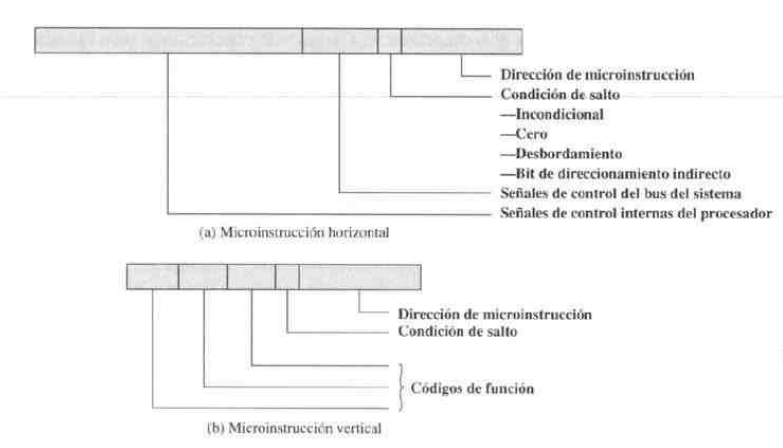
\includegraphics[scale=0.3]{imagenes/microinstruccion.png} 
	\end{figure}
\end{frame}


\begin{frame}
	\frametitle{Conceptos básicos}
	\begin{block}{Unidad de control microprogramada}
	Los elementos más importantes de esta implementación son:
	\begin{enumerate}
		\item \textbf{Memoria de control:} Almacena el conjunto de instrucciones
		\item \textbf{Registro de dirección de control:} Contiene la siguiente microinstrucción a leer
		\item \textbf{Registro intermedio de control:} Recibe la instrucción que se lee en memoria de control
	\end{enumerate}
	De este modo es suficiente con leer una microinstrucción en memoria para ejecutarla
	\end{block}	
	
\end{frame}

\begin{frame}
	\frametitle{Conceptos básicos}
	\begin{block}{Memoria de control}
	En la siguiente figura se puede observar la estructura de la memoria de control:
	\end{block}	
	\begin{figure}[H]
		\centering
		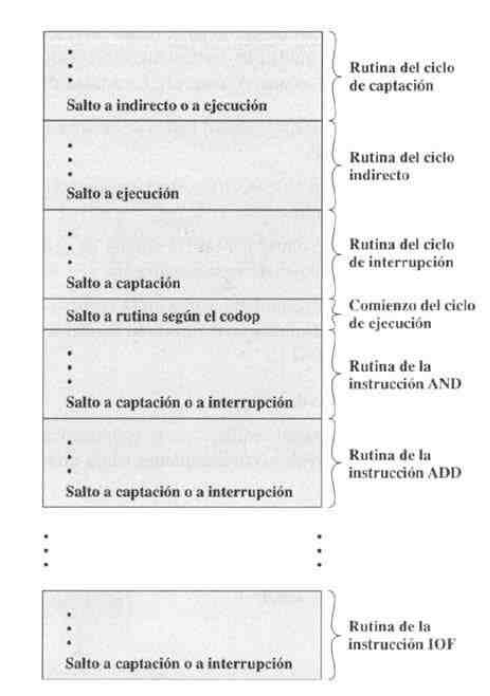
\includegraphics[scale=0.2]{imagenes/memoriacontrol.png} 
	\end{figure}
\end{frame}

\begin{frame}
	\frametitle{Conceptos básicos}
	\begin{block}{Memoria de control}
	En la siguiente figura se puede observar la organización de la memoria de control:
	\end{block}	
	\begin{figure}[H]
		\centering
		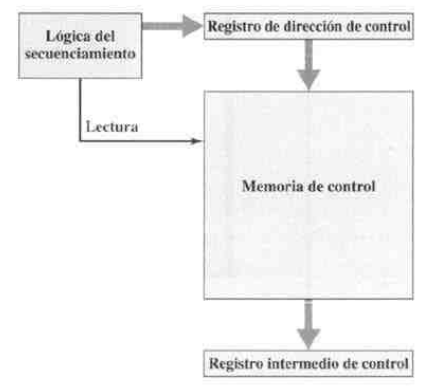
\includegraphics[scale=0.4]{imagenes/organizacionmemoriacontrol.png} 
	\end{figure}
\end{frame}

\begin{frame}
	\frametitle{Conceptos básicos}
	\begin{block}{Funcionamiento unidad de control}
	La unidad de control funciona de la siguiente forma:
	\begin{enumerate}
		\item La unidad de lógica de secuenciamiento emite una orden de lectura de memoria de control
		\item La palabra cuya dirección se especifica en el registro de control se lee en el registro intermedio de control
		\item El registro intermedio de control genera las señales de control y la información de dirección de la sugiente instrucción de control
		\item La unidad de lógica de secuenciamiento carga el registro de dirección de control una nueva dirección, basada en la información de instrucción siguiente y los indicadores de la ALU
	\end{enumerate}
	\end{block}	
	
\end{frame}


\begin{frame}
	\frametitle{Conceptos básicos}
	\begin{block}{Ventajas e inconvenientes}
	\begin{enumerate}
		\item La implementación microprogramada tiene un diseño más simple que la cableada, por ello es más barata y también permite adaptarla a los cambios tecnológicos
		\item El principal inconveniente es que la implementación microprogramada es más lenta que la cableada, debido a que la estructura de creación y procesamiento de microinstrucciones, frente al caso de la cableada donde sólo se requiere enviar la señales de control para la ejecución de las microoperaciones
	\end{enumerate}
	\end{block}		
\end{frame}




\section{Secuenciamiento de microinstrucciones}

\begin{frame}
	\frametitle{Secuenciamiento de microinstrucciones}
	\begin{block}{Conceptos}
	Las dos tareas básicas realizadas por una unidad de control microprogramadas
	\begin{enumerate}
		\item \textbf{Secuenciamiento de microinstrucciones:} Obtener la siguiente instrucción de la memoria de control
		\item \textbf{Ejecución de microinstrucciones:} Generar la señales de control necesarias para ejecutar la microinstrucción
	\end{enumerate}
	\end{block}	
\end{frame}


\begin{frame}
	\frametitle{Secuenciamiento de microinstrucciones}
	\begin{block}{Técnicas de secuenciamiento}
	A partir de la microinstrucción actual se debe generar la dirección de la siguiente microinstrucción. Debido a esto se agrupan las técnicas en estas tres categorías
	\begin{enumerate}
		\item \textbf{Dos campos de dirección:} Existe un multiplexor que permite elegir entre dos posibles direcciones para la microinstrucción, esto para dar soporte a los saltos
		\item \textbf{Un campo de dirección:} Al añadir un registro de dirección de control se puede reducir las direcciones a una, donde el multiplexor puede elegir entre la dirección de la siguiente instrucción o una dirección de salto en este registro
	\end{enumerate}
	\end{block}	
\end{frame}

\begin{frame}
	\frametitle{Secuenciamiento de microinstrucciones}
	\begin{block}{Técnicas de secuenciamiento}
	A partir de la microinstrucción actual se debe generar la dirección de la siguiente microinstrucción. Debido a esto se agrupan las técnicas en estas tres categorías
	\begin{enumerate} \setcounter{enumi}{2}
		\item \textbf{Formato variable:} Se puede determinar usar diferentes tipos de instrucción, donde un bit determina que tipo de instrucción se va utilizar. En un formato, la dirección es la siguiente microinstrucción y en el otro formato se puede especificar un salto. El inconveniente de esta implementación es que es más lenta que las dos anteriores.
	\end{enumerate}
	\end{block}	
\end{frame}

\begin{frame}
	\frametitle{Secuenciamiento de microinstrucciones}
	\begin{block}{Técnicas de secuenciamiento}
	Para el caso de dos campos de dirección
	\end{block}	
	\begin{figure}[H]
		\centering
		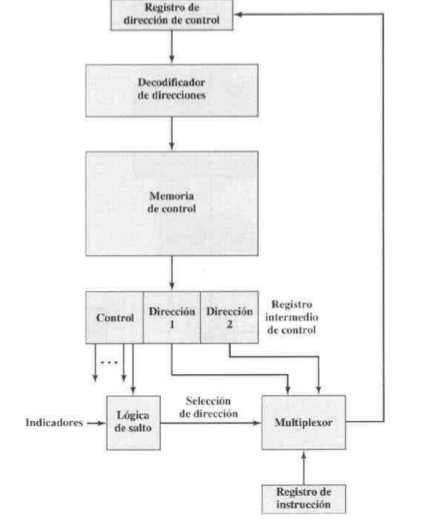
\includegraphics[scale=0.3]{imagenes/doscampos.png} 
	\end{figure}
\end{frame}

\begin{frame}
	\frametitle{Secuenciamiento de microinstrucciones}
	\begin{block}{Técnicas de secuenciamiento}
	Para el caso de un campo de dirección
	\end{block}	
	\begin{figure}[H]
		\centering
		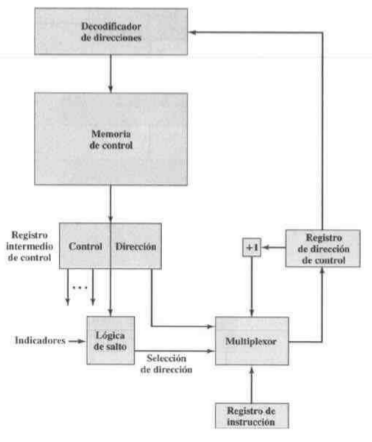
\includegraphics[scale=0.3]{imagenes/uncampo.png} 
	\end{figure}
\end{frame}

\begin{frame}
	\frametitle{Secuenciamiento de microinstrucciones}
	\begin{block}{Técnicas de secuenciamiento}
	Para el caso de formato variable
	\end{block}	
	\begin{figure}[H]
		\centering
		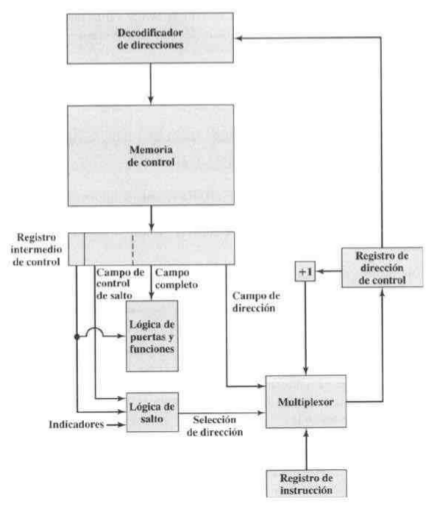
\includegraphics[scale=0.3]{imagenes/variable.png} 
	\end{figure}
\end{frame}


\begin{frame}
	\frametitle{Secuenciamiento de microinstrucciones}
	\begin{block}{Generación de direcciones}
	Estudiando el enfoque de una dirección, se puede estudiar como generar las direcciones para la siguiente microinstrucción o de un salto que depende de:
	\begin{enumerate}
		\item Indicadores de la ALU
		\item Modo de direccionamiento utilizado
		\item Partes de un registro, como el bit del signo
		\item Bits de estado en la unidad de control
	\end{enumerate}
	\end{block}	
\end{frame}

\begin{frame}
	\frametitle{Secuenciamiento de microinstrucciones}
	\begin{block}{Generación de direcciones}
	La técnica habitual consiste en combinar o sumar dos partes de una dirección para formar una dirección completa.
	\end{block}	
\end{frame}


\section{Ejecución de microinstrucciones}

\begin{frame}
	\frametitle{Ejecución de microinstrucciones}
	\begin{block}{Conceptos}
	El ciclo de microinstrucción es el evento básico de un procesador microprogramado. Cada ciclo consta de dos partes: Captación y Ejecución.
	\begin{itemize}
		\item En el ciclo de captación se genera una dirección de microinstrucción
		\item En el ciclo de ejecución se generan las señales de control para realizar la ejecución de la microinstrucción
	\end{itemize}
	\end{block}	
\end{frame}

\begin{frame}
	\frametitle{Ejecución de microinstrucciones}
	\begin{block}{¿Cómo se pueden codificar instrucciones?}
	Suponiendo existen $k$ señales de control se pueden generar $2^K$ combinaciones posibles de señales, sin embargo no todas las combinaciones son válidas, por ejemplo:
	\begin{itemize}
		\item Dos fuentes no pueden llevar al mismo destino
		\item Un registro no puede ser fuente y a la vez destino
		\item Sólo un patrón de señales de control a la ALU
		\item Sólo un patrón de señales de control puede presentar al bus de control cada vez
	\end{itemize}
	Por lo que se pueden reducir las combinaciones posibles, para utilizar los bits enteramente necesarios.
	\end{block}	
\end{frame}

\begin{frame}
	\frametitle{Ejecución de microinstrucciones}
	\begin{block}{¿Cómo se pueden codificar instrucciones?}
	Espectro de microinstrucciones:
	\end{block}	
	\begin{figure}[H]
		\centering
		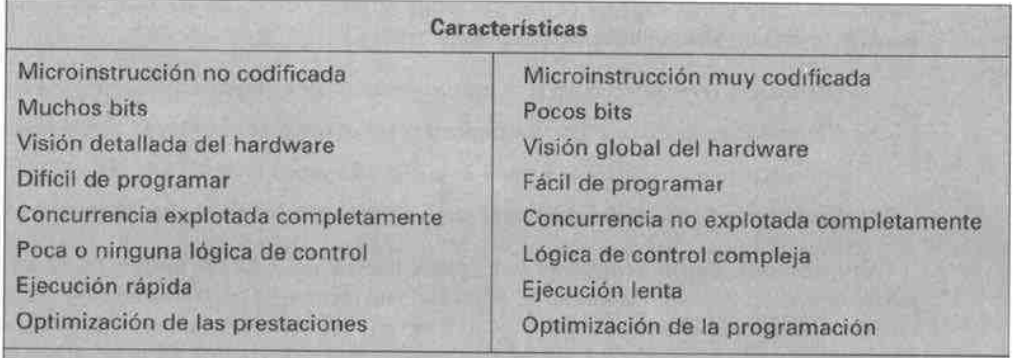
\includegraphics[scale=0.25]{imagenes/espectro.png} 
	\end{figure}
\end{frame}

\begin{frame}
	\frametitle{Ejecución de microinstrucciones}
	\begin{block}{¿Cómo se pueden codificar instrucciones?}
	Para reducir el tamaño de la memoria de control y simplificar la tarea de microprogramación, la microinstrucción se organiza como un conjunto de campo, cada campo tiene un código que, tras decodificar, activa una o más señales de control. Existen dos tipos de decodificación:
	\begin{enumerate}
		\item \textbf{Directa}: Cada campo se codifica directamente
		\item \textbf{Indirecta}: cada campo puede ser codificado directamente o junto a otros campos
	\end{enumerate}
	\end{block}	
\end{frame}

\begin{frame}
	\frametitle{Ejecución de microinstrucciones}
	\begin{block}{¿Cómo se pueden codificar instrucciones?}
	Caso de codificación directa
	\end{block}	
	\begin{figure}[H]
		\centering
		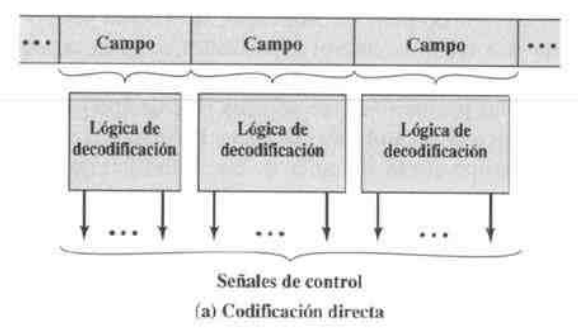
\includegraphics[scale=0.35]{imagenes/directa.png} 
	\end{figure}
\end{frame}

\begin{frame}
	\frametitle{Ejecución de microinstrucciones}
	\begin{block}{¿Cómo se pueden codificar instrucciones?}
	Caso de codificación indirecta
	\end{block}	
	\begin{figure}[H]
		\centering
		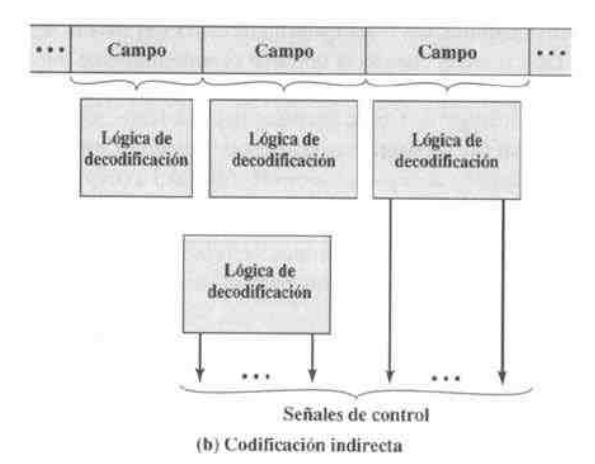
\includegraphics[scale=0.3]{imagenes/indirecta.png} 
	\end{figure}
\end{frame}
 
\section{Extra: BIOS} 

\begin{frame}
	\frametitle{Extra: BIOS}
	\begin{block}{Definiciones}
	\begin{itemize}
		\item BIOS significa Basic Input/output System,
		\item Es un programa especial, que se pone en marcha al encenderse el PC
		\item La BIOS no se carga como si de un sistema operativo 
		\item Viene incorporada a la placa base en un chip de memoria PROM o Flash.
	\end{itemize}
	\end{block}	
\end{frame}

\begin{frame}
	\frametitle{Extra: BIOS}
	\begin{block}{Definiciones}
		Memoria PROM o Flash de la BIOS
	\end{block}	
	\begin{figure}[H]
		\centering
		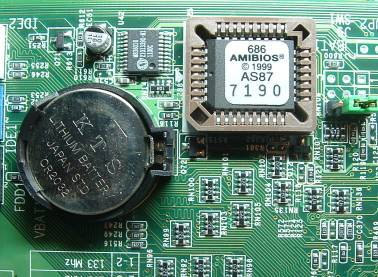
\includegraphics[scale=0.4]{imagenes/bios.jpg} 
	\end{figure}
\end{frame}


\begin{frame}
	\frametitle{Extra: BIOS}
	\begin{block}{Funcionalidades}
	\begin{itemize}
		\item Comprueba que todos los periféricos funcionan correctamente
		\item Verifica el tipo y el funcionamiento del disco duro
		\item Chequea el estado de la Memoria 
		\item Las BIOS pueden ser actualizadas por software, pero no pueden cambiarse, para hacerlo es necesario cambiar el chip
	\end{itemize}
	\end{block}	
\end{frame}


\begin{frame}
	\frametitle{Extra: BIOS}
	\begin{block}{Configuraciones}
	\begin{itemize}
		\item No comprobar disco duro ni memoria ni comprobar estado de periféricos
		\item Se puede habilitar o no virtualización en la CPU
		\item Cambiar el modo de administración de periféricos: DMA o E/S Programado
	\end{itemize}
	\end{block}	
\end{frame}

 
\begin{frame}
	\frametitle{Preguntas}
	\vfill
	\begin{center}
	¿Preguntas?\\
	\vfill
	Esto es todo, éxitos en el exámen
	\end{center}
\end{frame}


\end{document}